\documentclass[11pt]{article}
\usepackage{geometry}
\usepackage{graphicx}
\usepackage{array}
\usepackage{rotating}
\usepackage{pdflscape}
\usepackage{amsmath}
\numberwithin{figure}{section}
\numberwithin{table}{section}

%border spacing
\geometry{
 a4paper,
 lmargin = 1in,
 rmargin = 1in,
 tmargin = 1in,
 bmargin = 1in 
 }
 
%line spacing
\renewcommand{\baselinestretch}{1.5}  

\begin{document} 

\begin{titlepage}
	
	\centering
	\renewcommand{\baselinestretch}{1.7}\normalsize
	
	{\fontsize{1cm}{1.2em}\selectfont \scshape elephant detection and localization using infrasound}
	
	\vspace*{2\baselineskip}	
		
	\renewcommand{\baselinestretch}{1.25}\normalsize
	
	\vspace*{2\baselineskip}
	
	{by}
	
	\vspace*{0.3\baselineskip}
	{\Large K.K.T.P Ranathunga}
	\vspace*{0.3\baselineskip}
	
	{\itshape (Registration No : 2012/CS/112, Index No : 12001122)}
	
	{\normalsize tharindu.prf@gmail.com}
	
	\vspace*{2\baselineskip}
	
	\normalsize  {{Submitted in partial fulfillment}
		
		{Of the requirements of the}
		
		{B.Sc in Computer Science 4th Year Individual Project}
		
		{(SCS4124)}}
	
	\vspace*{2\baselineskip}
	
	
\includegraphics[scale=0.1]{ucsc.png}
	
	\vfill    
	
	{Supervised by}
	
	\vspace*{0.3\baselineskip}
	
	{\Large Dr. Chamath Keppitiyagama}
	

	
	%  \begin{small}
	%  {BSc (Colombo)}
	%	\end{small}   
	\vspace*{0.5\baselineskip}
	
	
	
	\vfill
	
	{University of Colombo School of Computing\\
		Colombo 7\\
		SRI LANKA}
	
	\vfill
	{November 11, 2016}
	%	\today 
	


\end{titlepage}
\pagenumbering{arabic}

\newpage
\section*{Chapter 01: Introduction.}
\subsection{Goal and objectives.}
\paragraph{}
The world elephant population has been on the decline \cite {13} due to many reasons, among which the human elephant conflict is a major cause. Human settlements and cultivations adjoining the forest areas have resulted in the blocking of elephant migration routes and further  the presence of crops attracts wild elephants, causing damages to livelihood of humans while threatening the lives of both elephants and humans. The wildlife conservation authorities worldwide do not possess an established method to manage this situation which is non-destructive to both elephants and humans, with most authorities having to resort to brute force, often consequently aggravating the situation in the long term \cite {13}. At present, the primary solution introduced is the use of electric fences around elephant habitats to prevent elephants venturing beyond their habitat to encroach into human settlements; an expensive and potentially life threatening solution. 
\paragraph{}
The objective of this research is to implement  a cost effective input to a larger system that will help to solve the human elephant conflict building on and expanding upon the previous findings of related research. Research to date has found that elephants pass various messages using infra sound frequencies and this low frequency sound waves travel a greater distance than higher frequency waves  due to high frequency waves being more easily absorbed by air molecules compared to the lower frequency waves \cite {5}. In this research, an electronic system consisting of low cost sensors that have the capability of detecting infrasound calls emitted by the elephants as well as digital signal processing techniques are combined to  identify elephant  infrasonic vocalizations to localize the sound emitting sources. Further, attempts are made to use these information in various scenarios such as prior warning system before elephants enter a cultivation and elephant herd detection among other things.

\subsection{Research question.} 
\paragraph{}
This research attempt to develop a method to distinguish an elephant call in a stream of sound data and to find an effective method of infrasound source localization using the phase difference of two infrasound waves captured by several sensors placed in different distances from the sound source. The research aims to answer two basic questions using a low cost sensor system consisting of off the shelf microphones capable of capturing infrasound:

\begin{enumerate}
\item How to identify an elephant call in an infrasound wave ? 
\item How to  localize a source emitting infrasound in a noisy environment ?
\end{enumerate}


\subsection{Background and Significance.} 

\paragraph{}
A typical human male voice in speech fluctuates around 110 Hertz, a female's voice at around 220 Hz and a child's at around 300 Hz. Among elephants, a typical male rumble fluctuates around a minimum of 12 Hz (more than 3 octaves below a man's voice), a female's rumble at around 13 Hz and a calf's around 22 Hz \cite {1} \cite {2}. In Asian elephants, this value fluctuates between 14 Hz to 24 Hz within 10 to 25 seconds \cite {3} due to their smaller vocal cords compared to African elephants.  Elephants produce a wide range  of sounds from very low frequency rumbles to higher frequency snorts, barks, roars, cries as well as many other type of  calls. 

\paragraph{}
Audio waves below 20 Hz frequency is considered as Infrasonic waves \cite {4}. As such, elephant rumbles can be considered as infrasonic waves and these rumbles follow all the properties of infrasonic waves. A significance of infrasonic waves is that it travels further than high frequency waves. Sound is a pressure wave vibration of molecules and as a result, whenever molecules move, there is an inevitable loss of energy as heat. As a result, sound is lost by heating the medium through which it propagates. Sound wave attenuation is frequency dependent in most media.

\begin{figure}[h]
\centering
image
\caption{Sound absorption coefficient per atmosphere for air at 20 degree Celsius according to relative humidity per atmosphere.\cite{14}}
\label{fig:logo}
\end{figure}

\paragraph{}
The above image \ref{fig:logo} is a graph displaying the attenuation of sound at difference frequencies \cite {5}, which shows that low frequency waves have low absorption coefficient. Therefore, low frequencies are not absorbed well and travel further than high frequencies. This property of infrasound waves can be used  for the acoustic detection of the wave from a greater distance from the source of the sound. The low-frequency sounds used by elephants for long-range communication travel a distance that exceeds 1 km \cite {3}. As mentioned in the objectives, this research focusses on detecting elephant infrasonic calls from long distance and localizing them. Detecting and localizing elephants is an essential component of any viable solution to human elephant conflict. Attempts towards acoustic detection and localization of elephants exist in literature. However, due to high cost in infrasonic sensors and complexity in detection of these signals  in noisy environment, no system exists to date, that operation ready in the field.

\paragraph{}
Various types of devices which are capable of capturing infrasonic waves exist and they were mostly used for detecting geographical phenomena such as earthquakes and volcanic eruptions. One such device used by most related research is Infitec Infra 20, which has a sampling rate of 50Hz. This device can be considered as a low cost infra sound recorder compared to other existing devices and this costs US\$ 345 \cite {7}. A significance of the research is the attempt to use a laboratory made sensor system which cost only US\$ 15, which is capable of recording at a sampling rate of 44100 Hz. This sensor system consists of a Panasonic Omnidirectional Back Electret Condenser Microphone \cite{15} (Model WM-64C/WM-64K), LM358 IC for amplifying and a low pass filter\cite{16}.This sensor has the ability to capture infrasonic waves from a lower bound of 0 Hz to an approximate upper bound of 150 Hz.


\paragraph{}
The second research question is based on infrasound localization, which can be done by measuring physical quantities like sound pressure and particle velocity. The best localization technique which is used by nature (Animal sound localization) can be applied to this context in localizing a sound source digitally. Humans as well as most other land-living vertebrates use the time delay between the arrival of a sound wave at each ear to discern the direction of the source \cite {8}. Similarly, localization can be done digitally by calculating the inter-aural time delay  between two microphones lying on a specified distance, which will be further explained in the research methodology. Potential problems include the detection in noisy environment, sparsity and irregularity of elephant call and pattern recognition. These problems will be addressed using advanced digital signal processing techniques and the knowledge based on the existing literature.

\subsection{Scope of the thesis.}
\paragraph{}
As the final outcome, my intention is to introduce a low cost elephant detecting and localization system specialized for Asian countries using the sensor equipments made in the Sustainable Computing Research Group at University of Colombo School of Computing.

\begin{flushleft}
\text{This research attempts to:}
\end{flushleft}

\begin{itemize}

\item 	Identify an elephant call in the infrasound range with low latency.
\item 	Localizing an elephant call using the low cost sensors system consisting of a condenser microphone.
\end{itemize}

\newpage
\section*{Chapter 02 : Literature Review.}
\paragraph{}
Various research types exist in this specific domain. The experiments carried out by Katharine Payne, a researcher in the Bio acoustics Research Program at the Laboratory of Ornithology at Cornell University, show that elephants use infrasound in communication, which can be considered as the initial steps of all research work on this area. In 1984, she discovered that elephants communicate in low frequencies during her research carried out at the Portland Zoo. Further, her work with William Langbauer, Jr. and Elizabeth Thomas have shown that elephants were indeed making infrasonic calls. Subsequent studies, in association with Joyce Poole, William Langbauer, Cynthia Moss, Russell Charif, Rowan Martin and others, took place in Kenya, Namibia, and Zimbabwe, leading to the conclusion that elephants use their powerful deep calls in long distance communication [6] and elephants make these calls when coordinating family and larger group behaviors, when competing for resources and dominance, as well as when attracting mates and announcing reproduction. Large vocal cords of elephants were able to produce low frequency sound signals considered as rumbles, which were able to travel around 5 km in distance \cite {6}. It is also revealed that the rumbles audible to human ears, are the harmonic waves created from the infrasonic fundamentals.


\paragraph{}
There has been comparatively less study of communication in Asian elephants. Acoustic communication in the Asian elephant by Dr. Shermin de Silva, a  James Smithson Fellow at Smithsonian Conservation Biology Institute, can be considered as a comprehensive study on communication in Asian elephants, which was published in the Behaviour biological journal in 2010. She categorized acoustic features into 8 'single' calls, 5 'combination' calls and one possibly unique male call, for a total of at least 14 distinct call types \cite {19}. Her observations and conclusions are based on the data collected at Udawalawa national park, Sri Lanka during 2007 and 2008. It is mentioned that 7 out of 14 distinct call types (rumble, rev, roar, cry, bark, grunt, husky-cry) are made out of elephants Larynx and most of the fundamentals of these calls were found to be infrasonic. While African elephants were the main subjects of considerable amount of existing literature with majority of these focusing on elephant detection in noisy environment; the human elephant conflict is more of a burning issue in South Asian countries like India and Sri Lanka.As a result, in 2002, there was an attempt at implementing a sensor system that detects infrasonic calls of elephants in Sri Lanka.

\paragraph{}
Elephant infrasound have not been recorded in wild Asian elephants anywhere in Asia prior to this research project in Sri Lanka in 2002. The prototype introduced by the above research was able to supports four infrasound sensors and is capable of standard DSP functions such as archiving and filtering. Sound detection has a long history although it was not specified to elephant infrasound calls. Recent researches have shown that this is possible using a template based or feature based technique. Matched filter method where two spectrograms of the pattern template and the signal are directly mapped, is a straightforward mechanism for detecting a pattern in a signal. Although it was optimal when finding the occurrence of a template in a recorded signal, it is sub optimal in the presence of complex noise \cite {10}. Therefore, a novel spectro-temporal method for signal enhancement based on the structure tensor \cite {11} was introduced by a group of researchers at University of Vienna, Austria. 

\paragraph{}
There are many works related to sound localization using microphones. Many techniques and algorithms have been introduced during past decades to detect the direction of sound emitting source. These are mainly based on the following three type of principles.
\begin{enumerate}
\item Time difference of arrival, where the systems measure the difference in time between the signals received by the microphones to localize the sound source.
\item Direction of arrival, where the phase difference between the signals is used to locate the sound source \cite {20}.
\item Energy based sound localization, where the energy of sound wave decreases when the sound wave propagates in the air. By measuring the sound energy at different sensor locations, one may localize the sound source \cite {21}
\end{enumerate}

\paragraph{}
The most significant techniques is the time delay estimation, due to its simplicity and accuracy \cite {22}. Several research works have compared the algorithms such as cross correlation method \cite {23}, phase transform \cite {24} and maximum likelihood estimator \cite {25} used to estimate the time delay. There are instances where they have used two sensors or array of sensors for the localization, where; when number of sensors increases, the mean error generated becomes relatively low \cite {26}.

\paragraph{}
Results of the experiments in the form of simulation results \cite {26} show that all methods were able to estimate the time delay, where the peak position indicates the time delay estimation. However, the phase transformation method (PHAT) achieved a sharper peak than the other methods, which helps to estimate the real delay time more accurately in the real situation. The maximum likelihood method also achieved a sharp peak. Although cross correlation has the widest peak, it still can estimate the real time delay in the simulation conditions. Since these works can be directly incorporated to elephant call localization, we can guarantee that the accuracy of the localization results can be increased. As a result, we are able to select and use the most convenient and easily implemented method for the localization experiments. The environment of the localization scenario can result in the lagging of sound waves. As elephant localization is done in a forest environment, this is a factor that should be taken in to account. Many works have been done regarding the localization of sound in reverberation environment. The precedence effect describes the phenomenon, whereby echoes are spatially fused to the location of an initial sound, by selectively suppressing the directional information of lagging sounds (echo suppression). Echo suppression is a prerequisite for faithful sound localization in natural environments but its reliability depends on the behavioral context \cite {27}. These works can be integrated with our findings to be produce an accurate infrasonic localization. 

\paragraph{}
Although different literature exists with regard to acoustic detection of elephants and infrasound waves, there is no significant attempt towards an economically feasible solution for localizing Asian elephants through the use of infrasound calls, applicable to developing countries like Sri Lanka and India. The review will emphasize the importance towards a research on addressing the above problem.


Related works on :
\begin{itemize}
  \item Biological researches on elephant communication. 
  \item Behavior of infra sound waves.
  \item Sound localization.
  \item Signal classification.
  \item Acoustic detection of elephants.
  \item Infra sound recording devices
\end{itemize}

\newpage
\section*{Chapter 03 : Design and Methodology.}
\paragraph{}
As mentioned in the background, this research will not produce an ultimate machinery to detect and  localize elephants. Rather, it will be an input to a system of this calibre, which will increase the accuracy and also help validate the results of such a system. The first phase of the research will mainly focus on the infra sound localization from a relatively large distance.

\paragraph{}
Localization will be done using cross correlation. Two infrasonic sensors, 3m away from each other, are placed at different location away from an infra sound emitting source, which is a full range speaker with a larger membrane, capable of emitting low frequency sounds connected to a low frequency amplifier. A recorded sound clip of 15 seconds will be input to an automatic angle calculator program. Abstract overview of the above mentioned program is shown in figure \ref{d:anglecal}. Before localization is tested for elephant sounds in  forest environments, this will be tested at university premises taking recordings at different places. Main concern of this works will be identifying the factors responsible for the generated error. Results of the preliminary experiments regarding the localization are included in section 9.

\begin{figure}[h]
\centering
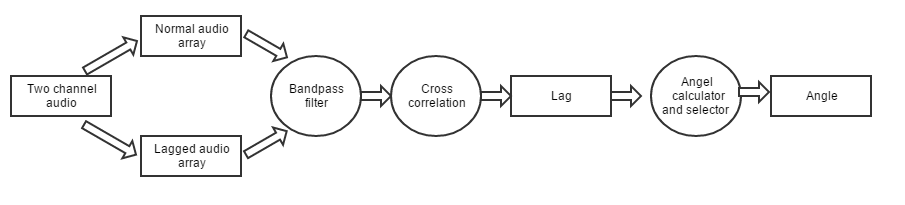
\includegraphics[width= \textwidth]{anglecal.png}
\caption{Overview of the cross correlation program}
\label{d:anglecal}
\end{figure}

\paragraph{}
A high level overview of the integrated components is given in figure \ref{d:H}. An input from the sensor system (recorded signal) will be pre-processed in order to smooth-en the signal wave. The sample rate of the recorded wave will be 44100. Feature extraction is performed to feed this data to the machine learning module. The purpose of this is to be done using MFCC (Mel-Frequency Cepstral coefficients) at the initial stage and Green-wood feature extraction in the secondary stage. 

\begin{figure}[h]
\centering
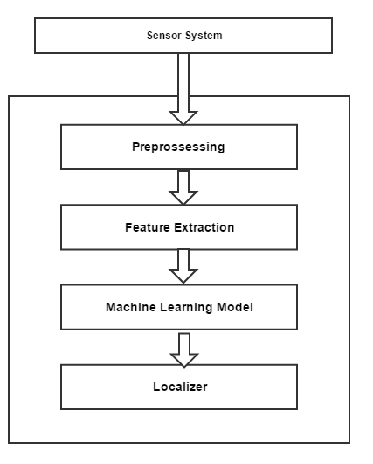
\includegraphics{flow.png}
\caption{High level overview of the integrated components}
\label{d:H}
\end{figure}

\paragraph{}
An appropriate machine learning model will be selected based on the conclusion of the existing work and using the data sets recorded at different forest areas in Sri Lanka as well as the data sets received from the Smithsonian biology conservation institute (SBCI), which will be used to train this machine learning model. There will be a comparison between the signal properties of the recorded audios by SBCI and our recordings using sensors made by us at the laboratory. In the next phase of the research, there will be an integration of the localization work and the pattern recognition work.

\paragraph{}
Since a main objective of this research is to produce a low cost sustainable solution, for elephant localization and detection, the quality of the results obtained using laboratory made components will also be compared against the high cost devices currently available.


\begin{itemize}
  \item Introducing Elocate sensors.
  \item Overview of sound localization. 
  \item Comparison of localization techniques.
  \item Application of cross correlation using Elocate sensors.
  \item Feature extraction.
  \item Signal enhancement.
  \item Classification using SVM.
\end{itemize}

\newpage
\section*{Chapter 04 : Implementation.}
\begin{itemize}
  \item Electronic circuit of the sensors.
  \item Noise reduction techniques.
  \item Implementation of localization.
  \item Data collection.
  \item Implementation of pre processing.
  \item Training SVM.
  \item Testing the model.
\end{itemize}
\section*{Chapter 05 : Results and Evaluation.}
\begin{itemize}
  \item Results of each experiment conducted.
  \item A comprehensive analysis on results.
\end{itemize}
\section*{Chapter 06 : Conclusion and Future Works.}
\begin{itemize}
  \item New possibilities discovered.
  \item Problems encountered.
  \item Increasing the accuracy of detection and localization.
  \item Summary
\end{itemize}
\newpage



\newpage
\begin{thebibliography}{1}
\bibitem{1} Berg, J.K. 1983. Vocalizations and associated behaviours of the African elephant Loxodonta africana in captivity. Z. Tierpsychol 63:63-79.
\bibitem{2}Payne, K. 2003. Sources of Social Complexity in the Three Elephant Species. In: Animal Social Complexity: Intelligence, Culture, and Individualized Societies. Ed: Frans B.M. de Waal and Peter L. Tyack. Harvard University Press.
\bibitem{3} Payne, K., Langbauer, Jr., W.R., and Thomas, E. 1986. Infrasonic calls of the Asian elephant (Elephas maximus). Behavioral Ecology and Sociobiology.
\bibitem{4} “Infrasonic Sound", Hyperphysics.phy-astr.gsu.edu, 2016. [Online]. Available: http://hyperphysics.phy-astr.gsu.edu/hbase/sound/infrasound.html. [Accessed: 27- Apr- 2016].
\bibitem{5} Szabo T. L., 1994, “Time domain wave equations for lossy media obeying a frequency power law,” J. Acoust. Soc. Am., 96(1), pp. 491-500.
\bibitem{6} Payne, K., Thompson, M., and Kramer, L. 2003. Elephant calling patterns as indicators of group size and composition: the basis for an acoustic monitoring system. African Journal of Ecology, 41: 99-107
\bibitem{7} "INFILTEC: The Inexpensive Infrasound Monitor Project. - simple microbarograph design for DIY", Infiltec.com, 2016. [Online]. Available: http://www.infiltec.com/Infrasound@home/. [Accessed: 27- Apr- 2016].
\bibitem{8} A. Vedurmudi, J. Goulet, J. Christensen-Dalsgaard, B. Young, R. Williams and J. van Hemmen, "How Internally Coupled Ears Generate Temporal and Amplitude Cues for Sound Localization",Phys. Rev. Lett., vol. 116, no. 2, 2016.
\bibitem{9} ] Larom, D., M. Garstang, K. Payne, R. Raspet \& M. Lindeque. 1997. The influence of surface atmospheric conditions on the range and area reached by animal vocalizations. J. Experimental Biol. 200: 421-431.
\bibitem{10} P. J. Venter and J. J. Hanekom. Automatic detection of african elephant (loxodonta africana) infrasonic vocalisations from recordings. Biosystems engineering.
\bibitem{11} Acoustic Detection of Elephant Presence in Noisy Environments Matthias Zeppelzauer Vienna University of Technology.
\bibitem{12} MUSIC Algorithm", Ptolemy.eecs.berkeley.edu, 2016. [Online]. Available: http://ptolemy.eecs.berkeley.edu/papers/96/dtmf\_ict/www/node5.html. [Accessed: 27- Apr- 2016].
\bibitem{13} Lalith Seneviratne, G. Rossel, W.D.C.. Gunasekera, H.L.P.A. Madanayake, Y.M.S.S. Yapa and G. Doluweera.Elephant Infrasound Calls as a Method for Electronic Elephant Detection.
\bibitem{14} J. E. Piercy, T. F. W. Embleton, L. C. Sutherland, Review of noise propagation in the atmosphere, J. Acoust. Soc. Am. Volume 61, Issue 6, pp. 1403-1418, June 1977.
\bibitem{15} Panasonic Corporation. Panasonic Omnidirectional Back Electret Condenser Microphone Cartidge.[2016].  [Online]. Available: http://industrial.panasonic.com/cdbs/www-data/pdf/ABA5000/ABA5000CE22.pdf. [Accessed: 28- Apr- 2016].
\bibitem{16}"LM358 | General Purpose Amplifier | Operational Amplifier (Op Amp) | Description \& parametrics", Ti.com, 2016. [Online]. Available: http://www.ti.com/product/LM358. [Accessed: 28- Apr- 2016].
\bibitem{17}Jean-Marc Valin, Franc¸ois Michaud, Jean Rouat, Dominic Letourneau LABORIUS - Research Laboratory on Mobile Robotics and Intelligent Systems Department of Electrical Engineering and Computer Engineering Universite´ de Sherbrooke.Robust Sound Source Localization Using a Microphone Array on a Mobile Robot.
\bibitem{18} Richard F. Lyon, Andreas G. Katsiamis, Emmanuel M. Drakakis (2010). "History and Future of Auditory Filter Models"
\bibitem{19} Shermin de Silva "Acoustic communication in the Asian elephant,
Elephas maximus maximus"
\bibitem{20} Taff, L. G, “Target Localization from Bearings-only Observations,”
IEEE Trans. Aerosp. Electron., 3, issue 1, (1997).New York: McGraw-Hill, 1964, pp. 15–64.
\bibitem{21}D.Li, and Y. H. Hu, “Energy Based Collaborative Source Localization
Using Acoustic Micro-Sensor Array,” EURASIP Journal on Applied
Signal Processing, vol. 2003, no. 4, pp. 321-337, 2003.
\bibitem{22}M. Brandstein and H. Silverman, “A Practical Methodology for Speech
Source Localization with Microphone arrays,” Comput., Speech Lng.,
vol. 11, no. 2, pp. 91-126, 1997.
\bibitem{23} G. C. Carter, “Tutorial Overview of Coherence and Time Delay Estimation,”
in Coherence and Time Delay Estimation—An Applied Tutorial for Research, Development, Test, and Evaluation Engineers, vol. 1,1993,pp. 1–27
\bibitem{24}C. H. Knapp and G. C. Carter, “The Generalized Correlation Method for Estimation of Time Delay,” IEEE Trans. Acoust., Speech, Signal Processing,vol. ASSP-24, pp. 320–327, Aug.1976.
\bibitem{25}  J.benesty, “Adaptive Eigenvalue Decomposition Algorithm for Passive Acoustic Source Localization,” Acoustical Society of America, January 2000.
\bibitem{26} Hasan Khaddour, "A Comparison of Algorithms of Sound Source Localization Based
on Time Delay Estimation"
\bibitem{27} Sasha Devore,Antje Ihlefeld,Kenneth Hancock,Barbara Shinn-Cunningham,Bertrand Delgutte,
"Accurate Sound Localization in Reverberant Environments Is Mediated by Robust Encoding of Spatial Cues in the Auditory Midbrain"
\end{thebibliography}

\end{document}